
\begin{figure}[H]
    \centering
    \begin{subfigure}[b]{0.49\textwidth}
        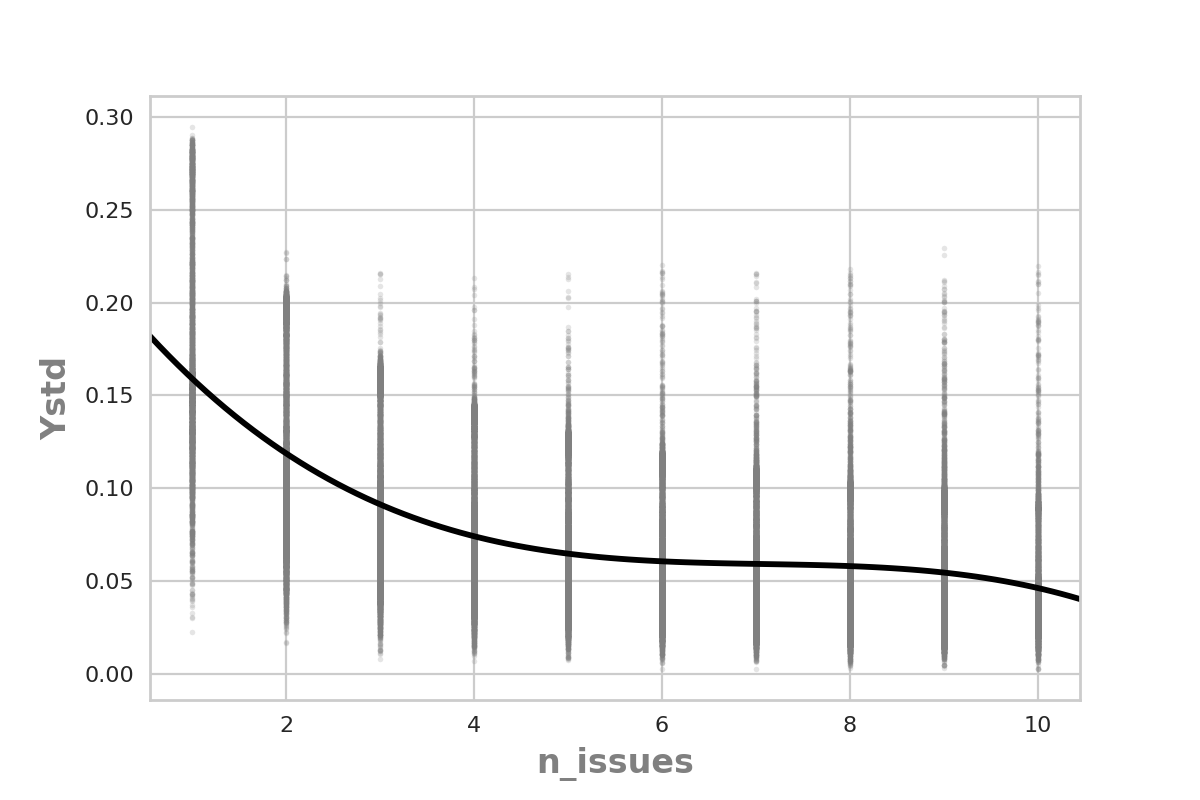
\includegraphics[width=\textwidth]{ims/nlregressions/nlregressionmutatingon_issues.png}
    \end{subfigure}
    \begin{subfigure}[b]{0.49\textwidth}
        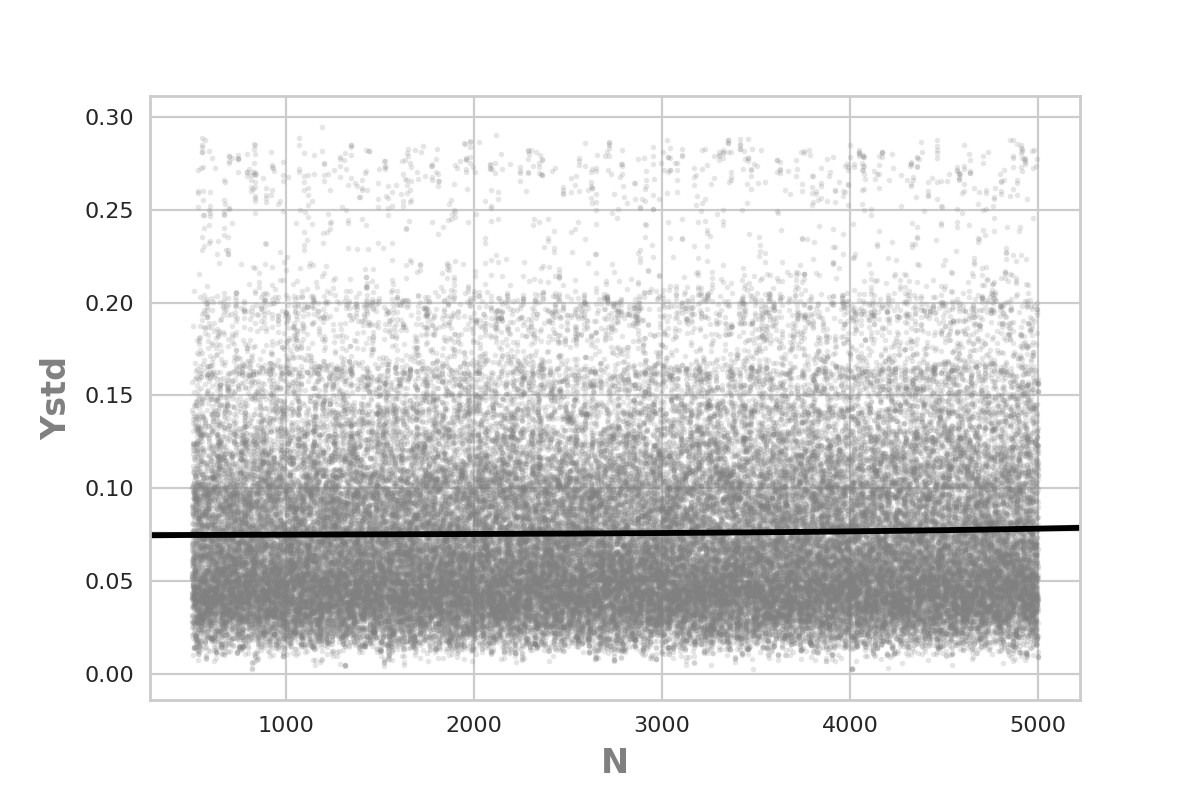
\includegraphics[width=\textwidth]{ims/nlregressions/nlregressionmutatingoN.png}
    \end{subfigure}

    \begin{subfigure}[b]{0.49\textwidth}
        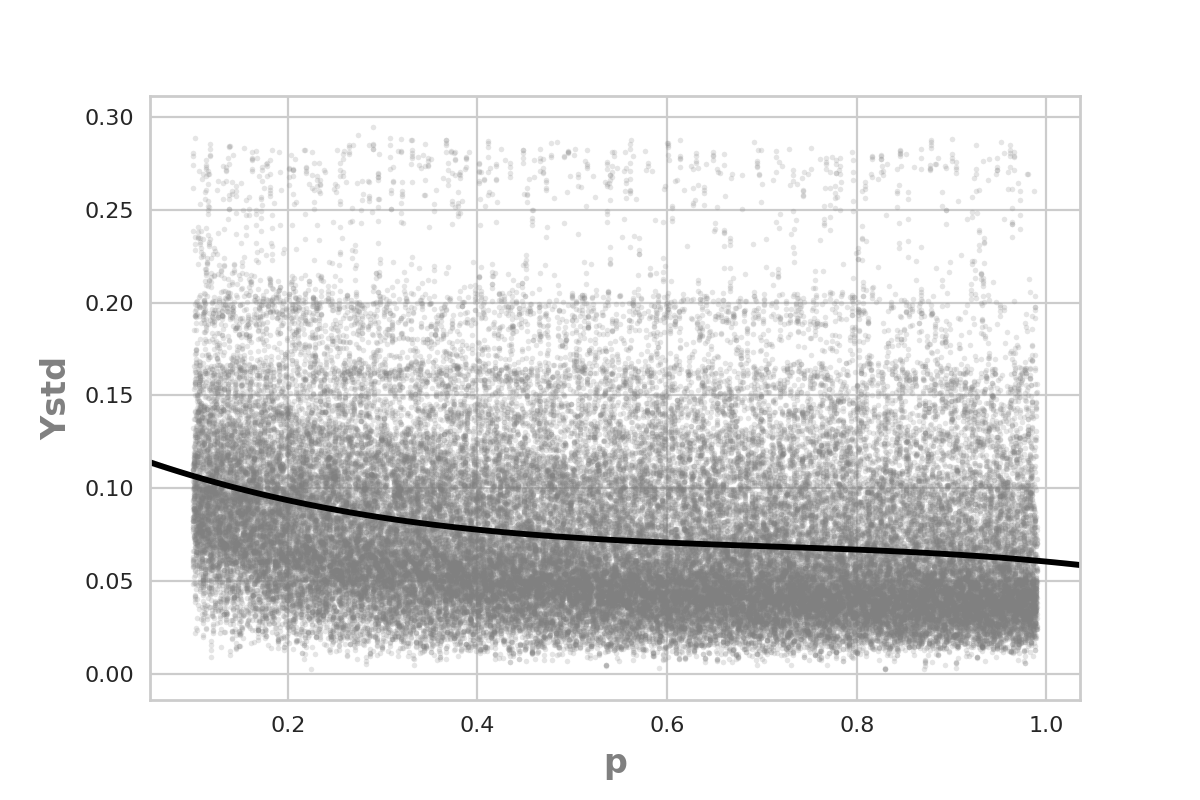
\includegraphics[width=\textwidth]{ims/nlregressions/nlregressionmutatingop.png}
      \end{subfigure}
          \begin{subfigure}[b]{0.49\textwidth}
            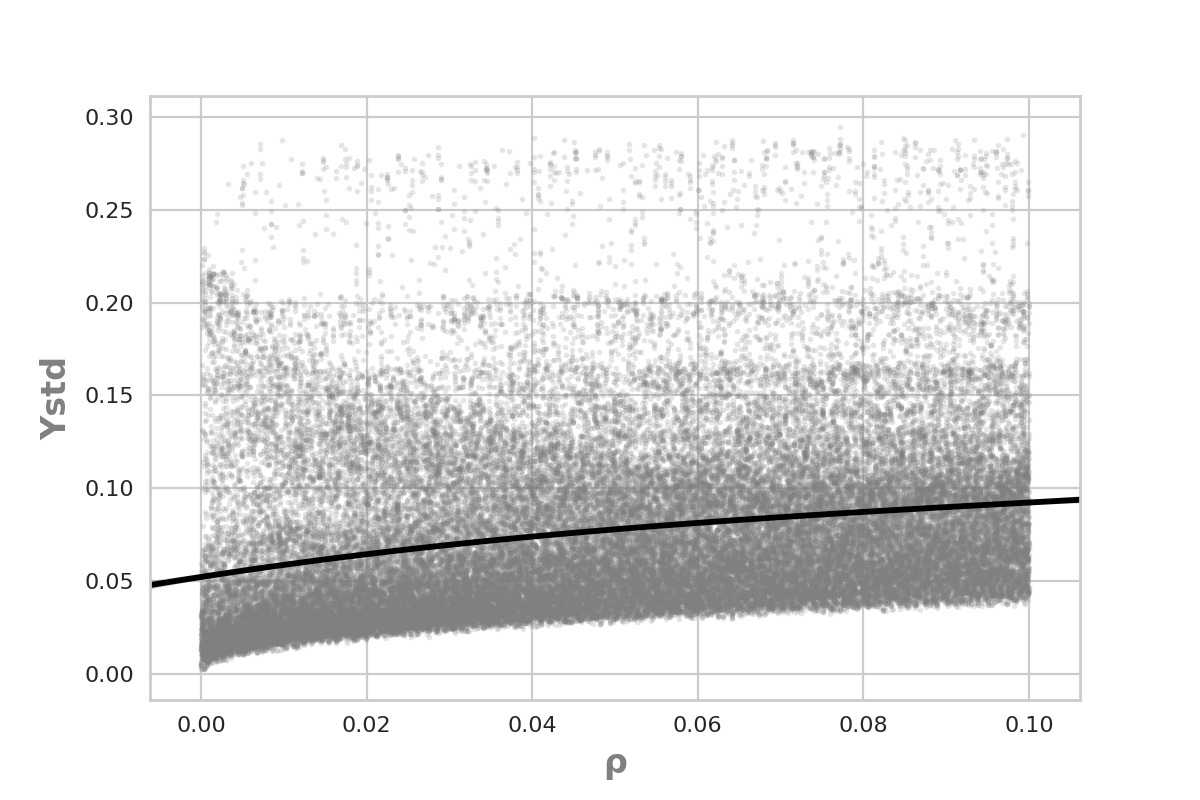
\includegraphics[width=\textwidth]{ims/nlregressions/nlregressionmutatingorho.png}
      \end{subfigure}

                \begin{subfigure}[b]{0.49\textwidth}
            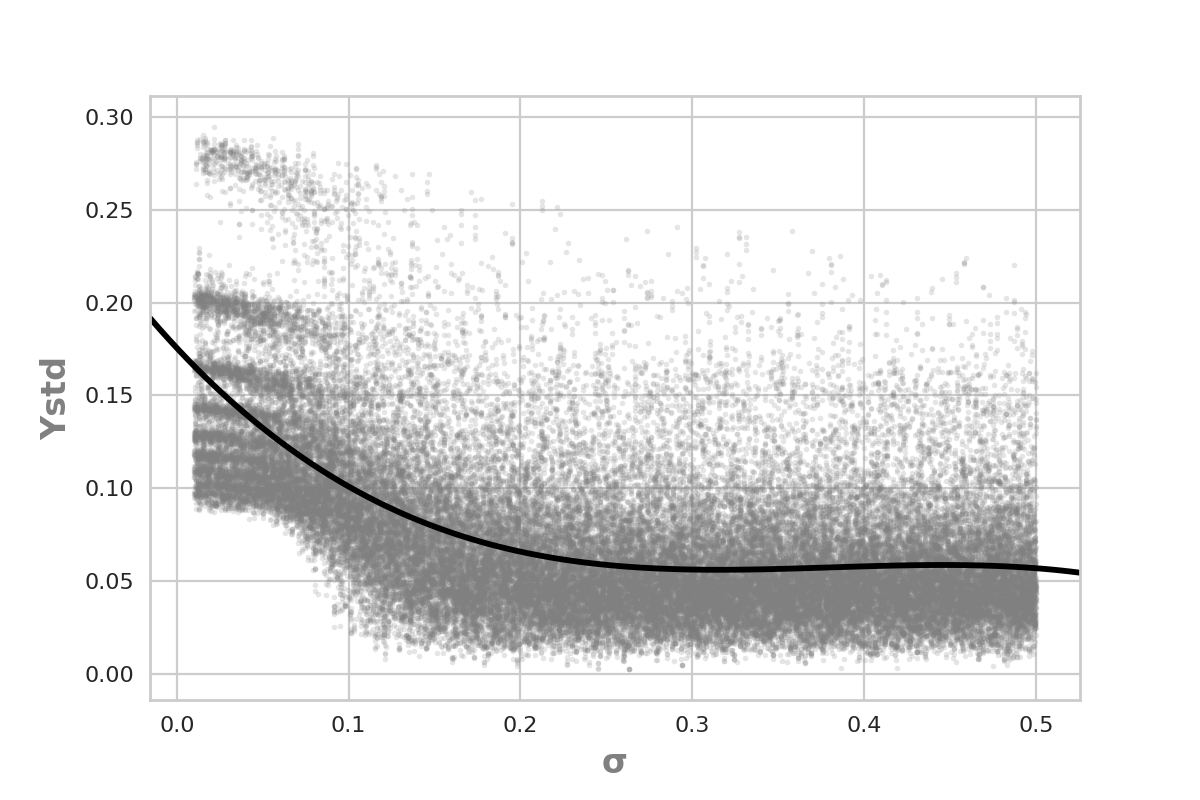
\includegraphics[width=\textwidth]{ims/nlregressions/nlregressionmutatingosigma.png}
          \end{subfigure}
                \begin{subfigure}[b]{0.49\textwidth}
            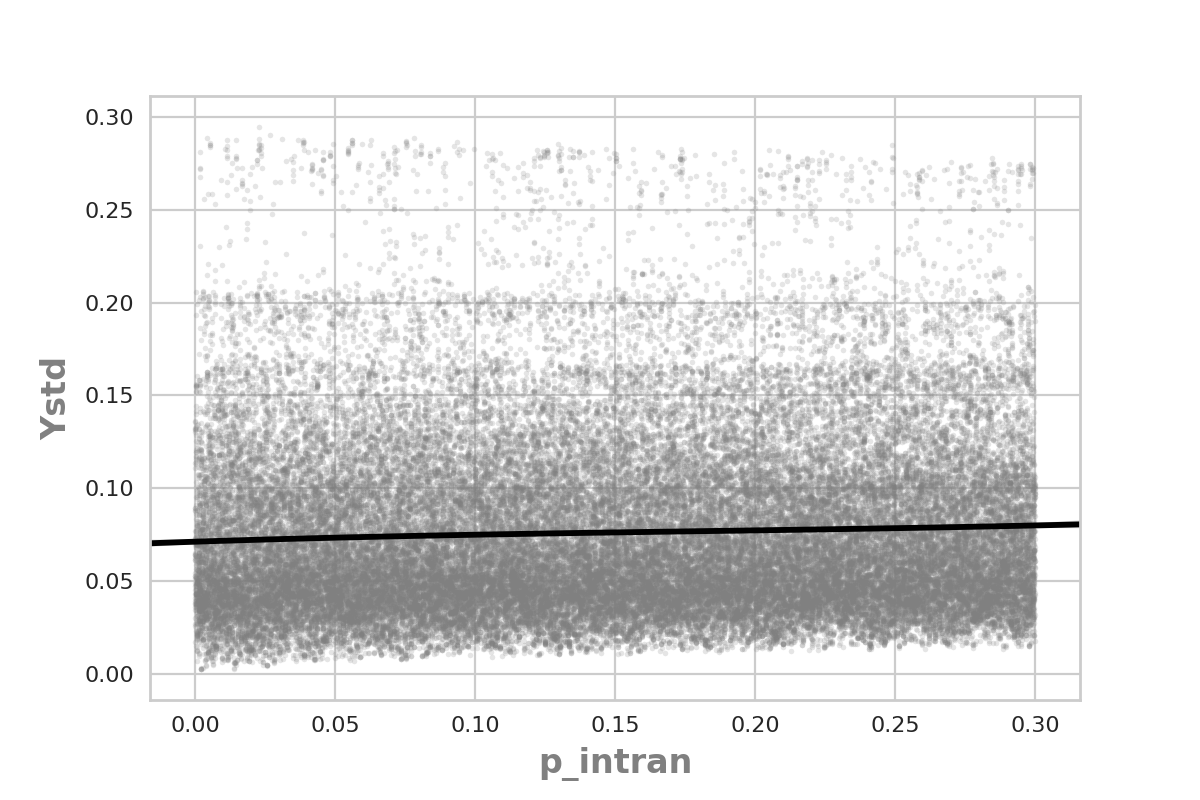
\includegraphics[width=\textwidth]{ims/nlregressions/nlregressionmutatingop_intran.png}
    \end{subfigure}
    \caption{Gráfico de dispersão e regressões polinomiais para 70.000 parametrizações.}
    \label{fig:scatter2}
    Fonte:Elaboração própria.
\end{figure}
%%% Local Variables:
%%% mode: latex
%%% TeX-master: "master"
%%% End:
